%##############################################################################
\chapter{Anhang zum Vorlesungsskript}
%##############################################################################
%
\begin{figure}
	\centering
	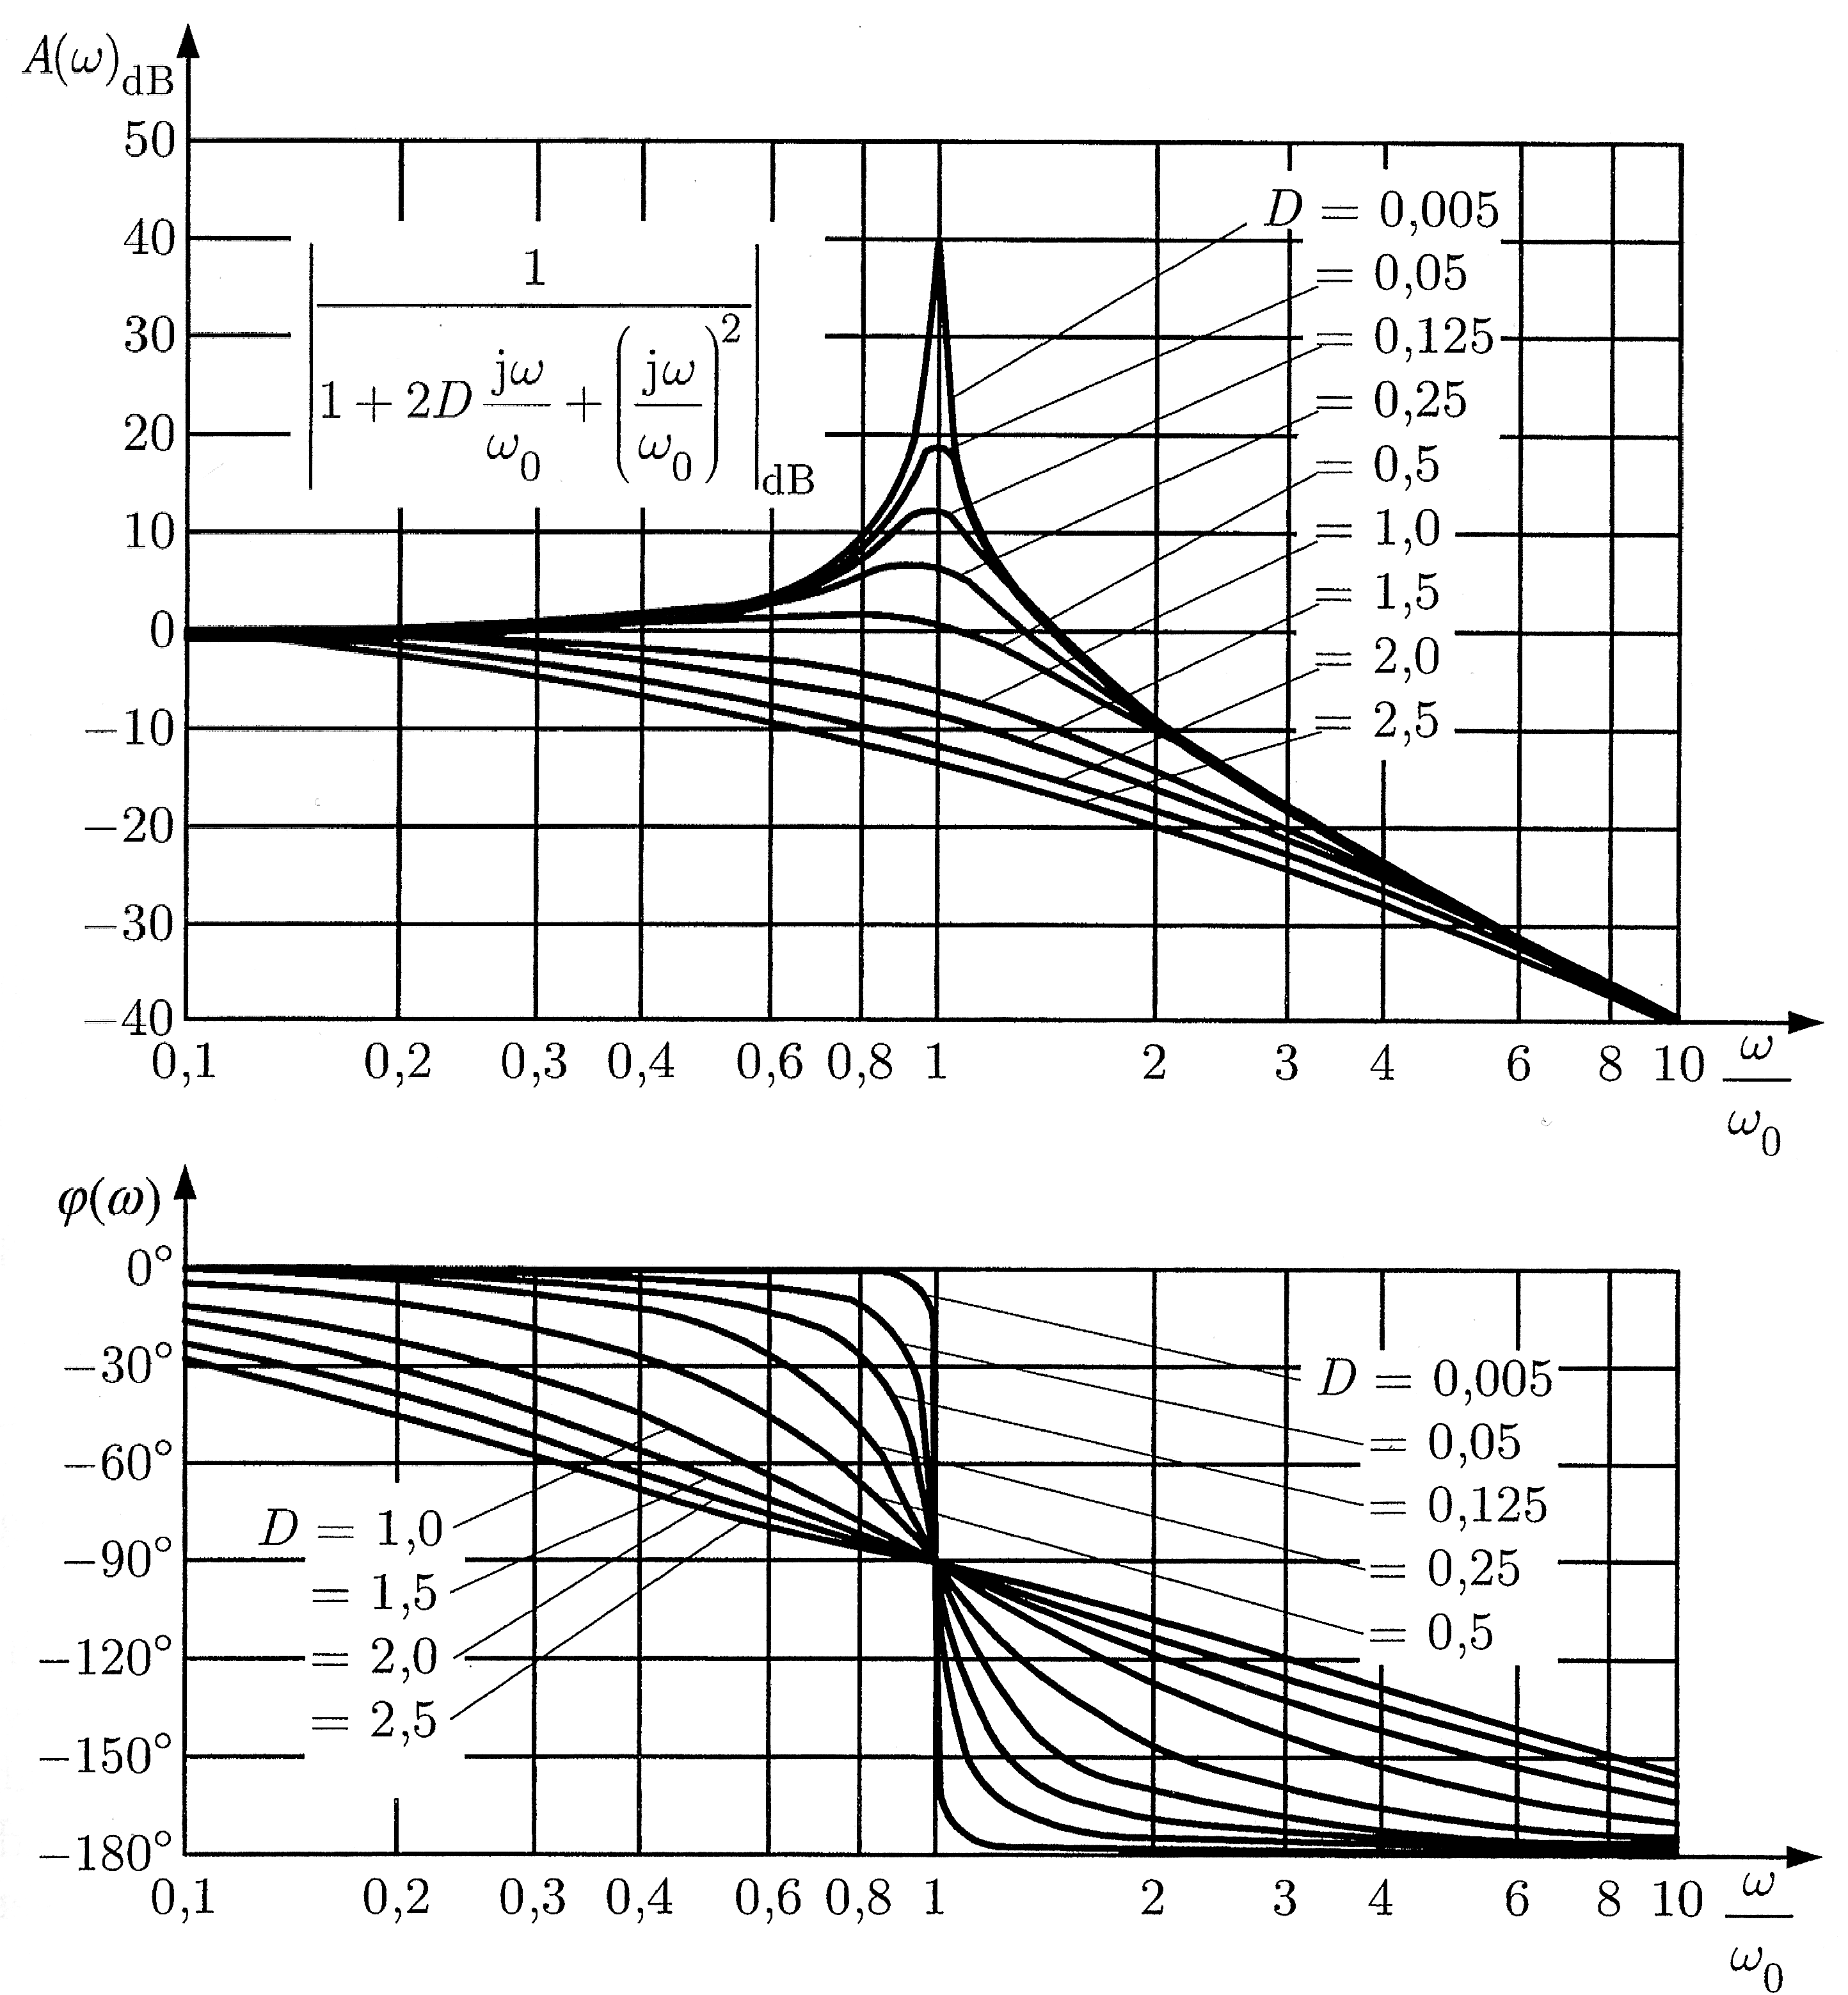
\includegraphics[width=0.9\linewidth]{Abbildungen/Anhang/FrequenzkennliniePT2}
	\caption{Bodediagramm eines PT$_{2}$-Gliedes für unterschiedliche Pollagen \cite{Unbehauen08}}
	\label{fig:pt2bode}
\end{figure}
%
\begin{figure}
	\centering
	\includegraphics[width=1\linewidth]{Abbildungen/Anhang/PT2Verhalten}
	\caption{Zeitverhalten eines PT$_{2}$-Gliedes für unterschiedliche Pollagen \cite{Unbehauen08}}
	\label{fig:pt2verhalten}
\end{figure}
%
\begin{figure}
	\centering
	\includegraphics[width=1\linewidth]{Abbildungen/Anhang/Rechenregeln_Laplace_Transformation}
	\caption{Rechenregeln der Laplacetransformation \cite{Winkler10}}
	\label{fig:LaplaceRegeln}
\end{figure}
%
\begin{table}
	%
	\centering
	%
	\begin{tabular}{|m{1cm}|m{5cm}|m{5cm}|} \hline
		%
		\textbf{Nr.} & \textbf{Zeitfunktion} & \textbf{Laplacebereich}\\ \hline\hline
		%
		1 & $\delta(t)$ & $1$\\\hline
		%
		2 & $\sigma(t)$ & $\frac{1}{s}$\\\hline
		%
		3 & $t$ & $\frac{1}{s^{2}}$\\\hline
		%
		4 & $t^{n}f(t)$ & $(-1)^{n}F^(n)(s)$\\\hline
		%
		5 & $f(at)$ mit a>0 & $\frac{1}{a}F(\frac{s}{a})$\\\hline
		%
		6 & $e^{-at}f(t)$ & $F(s+a)$\\\hline
		%
		7 & $e^{at}$ & $\frac{1}{s-a}$\\\hline
		%
		8 & $\frac{e^{\frac{t}{a}}}{a}$ & $\frac{1}{as-1}$\\\hline
		%
		9 & $\frac{e^{at}-1}{a}$ & $\frac{1}{s(s-a)}$\\\hline
		%
		10 & $t\,e^{at}$ & $\frac{1}{(s-a)^{2}}$\\\hline
		%
		11 & $\frac{e^{at}-e^{bt}}{a-b}$ & $\frac{1}{(s-a)(s-b)}$\\\hline
		%
		12 & $(1+at)e^{at}$ & $\frac{s}{(s-a)^{2}}$\\\hline
		%
		13 & $\frac{(at-1)e^{at}+1}{a^{2}}$ & $\frac{1}{s(s-a)^{2}}$\\\hline
		%
		14 & $\sin(at)$ & $\frac{a}{s^{2}+a^{2}}$\\\hline
		%
		15 & $\cos(at)$ & $\frac{s}{s^{2}+a^{2}}$\\\hline
		%
		16 & $e^{bt}\sin(at)$ & $\frac{a}{(s-b)^{2}+a^{2}}$\\\hline
		%
		17 & $e^{bt}\cos(at)$ & $\frac{s-b}{(s-b)^{2}+a^{2}}$\\\hline
		%
	\end{tabular}
	%
	\label{tab:GridSetupCigre}
	%
\end{table}
%

